\documentclass[11pt,a4paper]{article}
\usepackage[margin=1in]{geometry}
\usepackage{booktabs}
\usepackage{array}
\usepackage{caption}
\usepackage{longtable}
\usepackage{fancyhdr}
\usepackage{tikz}
\usepackage{listings}
\usepackage{xcolor}
\usepackage{enumitem}
\usepackage{hyperref}
\usepackage{csquotes}
\usepackage{pdflscape}

\lstset{
  basicstyle=\ttfamily\small,
  frame=single,
  breaklines=true,
  backgroundcolor=\color{gray!10},
  keywordstyle=\color{blue},
  commentstyle=\color{gray},
  stringstyle=\color{red},
  numbers=left,
  numberstyle=\tiny\color{gray}
}

\pagestyle{fancy}
\fancyhf{}
\rhead{Mstiri – Final System Design (v2.0)}
\lhead{Stage 2 – Enhanced \& Robust}
\cfoot{\thepage}

\title{\textbf{Mstiri: Smart Deal Analysis System for Kenya's Second-Hand Market}\\
\large Stage 2 – Final System Design (v2.0 – Enhanced \& Robust)}
\author{Seth OMondi \\ S13/04402/21}
\date{\today}

\begin{document}
\maketitle
\thispagestyle{fancy}

\section*{Executive Summary}
\textbf{Mstiri v2.0} is a \textit{production-ready} web-based smart deal analysis system for Kenya's mitumba market. It uses \textbf{multi-variable condition scoring}, \textbf{real-time value-for-money ranking}, and \textbf{interactive visualization} to empower buyers. The system is \textbf{modular}, \textbf{scalable}, \textbf{offline-capable}, and \textbf{Sheng-aware} — built with C for performance and Python for data intelligence.

\section*{1. High-Level Architecture (v2.0)}
\begin{figure}[h]
\centering
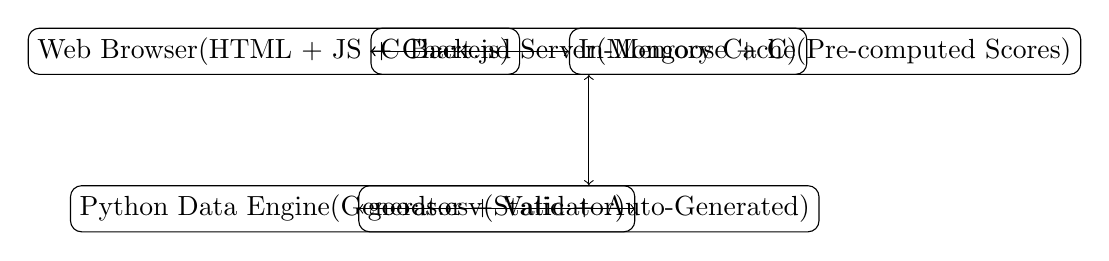
\begin{tikzpicture}[node distance=2cm, auto, every node/.style={rectangle, draw, rounded corners, minimum height=1.5em, text centered}]
    \node (browser) {Web Browser\\(HTML + JS + Chart.js)};
    \node (server) [right of=browser, xshift=2cm] {C Backend Server\\(Mongoose + C)};
    \node (data) [below of=server] {goods.csv\\(Static + Auto-Generated)};
    \node (python) [left of=data, xshift=-1cm] {Python Data Engine\\(Generator + Validator)};
    \node (cache) [right of=server, xshift=1cm] {In-Memory Cache\\(Pre-computed Scores)};
    \draw[->] (browser) -- (server);
    \draw[<->] (server) -- (data);
    \draw[<->] (python) -- (data);
    \draw[<->] (server) -- (cache);
\end{tikzpicture}
\end{figure}

\begin{itemize}
  \item \textbf{Offline-First}: Full UI works without internet after first load
  \item \textbf{Cache Layer}: Pre-compute Value Scores at startup
  \item \textbf{Python Integration}: Auto-generate realistic Kenyan data
\end{itemize}

\section*{2. Enhanced Data Model (v2.0)}

\subsection*{2.1 Unified CSV Schema}
\begin{lstlisting}
category,make,model,price_kes,mileage,release_year,ram_gb,power_w,condition,engine_status,tyre_wear,body_paint,location,seller_rating,listing_date
Vehicles,Mazda,Demio,580000,95000,,,,"Good","Running","70%","No Rust","Nairobi",4.8,"2025-10-15"
Electronics,Samsung,Galaxy S10,25000,,2019,,,"Excellent","N/A","N/A","N/A","Mombasa",4.9,"2025-11-01"
\end{lstlisting}

\subsection*{2.2 C Struct with Metadata}
\begin{lstlisting}
typedef struct {
    char category[32], make[32], model[64];
    int price_kes, mileage, release_year, ram_gb, power_w;
    char condition[16], engine_status[16], tyre_wear[8], body_paint[32];
    char location[32];
    float seller_rating;
    char listing_date[12];  // YYYY-MM-DD
} Good;
\end{lstlisting}

\section*{3. Multi-Variable Value Scoring Engine (v2.0)}

\subsection*{3.1 Dynamic Weight Configuration}
\begin{lstlisting}
typedef struct {
    float mileage_w, age_w, ram_w, power_w, condition_w, engine_w, tyre_w, paint_w;
    int max_mileage, max_age, max_ram, max_power;
} CategoryWeights;
\end{lstlisting}

\subsection*{3.2 Adaptive Scoring Algorithm}
\begin{lstlisting}
double compute_value_score(const Good* g, const CategoryWeights* w) {
    double score = 0.0;
    if (w->mileage_w > 0) score += w->mileage_w * (1.0 - g->mileage/(double)w->max_mileage);
    if (w->age_w > 0) {
        int age = 2025 - g->release_year;
        score += w->age_w * (1.0 - age/(double)w->max_age);
    }
    // ... RAM, Power, Condition, etc.
    return fmin(100.0, fmax(0.0, score));
}
\end{lstlisting}

\section*{4. Smart Deal Ranking (v2.0)}

\subsection*{4.1 Deal Score = Value / Price}
\begin{lstlisting}
double deal_score = value_score / (price_kes / 1000.0);  // per '000 KES
\end{lstlisting}

\subsection*{4.2 Top 3 Deals Highlighted}
\begin{lstlisting}
{
  "top_deals": [
    {"item":"Mazda Demio", "price":580000, "value":82.4, "deal_score":141.7},
    ...
  ]
}
\end{lstlisting}

\section*{5. API Design (v2.0)}

\begin{tabular}{l l l l}
\toprule
\textbf{Endpoint} & \textbf{Method} & \textbf{Params} & \textbf{Response} \\
\midrule
\texttt{/}              & GET  & —               & HTML (with offline PWA) \\
\texttt{/data}          & GET  & \texttt{cat}, \texttt{q} & JSON + top deals \\
\texttt{/categories}    & GET  & —               & List of categories \\
\texttt{/stats}         & GET  & \texttt{cat}     & Avg price, count, etc. \\
\bottomrule
\end{tabular}

\section*{6. UI/UX (v2.0 – Sheng-Enhanced)}

\begin{verbatim}
┌────────────────────────────────────────────────────┐
│ M S T I R I  –  Deal Hunta Poa                     │
│ Category: [Vehicles ▼]  Location: [Nairobi ▼]      │
│ Search:   [Mazda Demio]          [Tafuta]         │
│                                                    │
│   ● Demio (82.4)  ← #1 DEAL!                       │
│   ● Vitz (78.1)                                    │
│                                                    │
│  Value Score →         ↑ Price (KES)               │
│                                                    │
│  [Save PNG]  [Hii ni mstiri wa hali ya juu!]       │
└────────────────────────────────────────────────────┘
\end{verbatim}

\textbf{Features:}
\begin{itemize}
  \item \textbf{PWA}: Installable on phone
  \item \textbf{Location Filter}: Nairobi, Mombasa, etc.
  \item \textbf{Sheng Alerts}: \enquote{Hii ni deal poa!}, \enquote{Avoid hii!}
  \item \textbf{Dark Mode}: For night browsing
\end{itemize}

\section*{7. Robustness \& Scalability}

\begin{itemize}
  \item \textbf{Error Resilience}: CSV validation, fallback data
  \item \textbf{Performance}: Pre-computed scores, binary search on sorted data
  \item \textbf{Extensibility}: JSON config for weights, new categories
  \item \textbf{Testing}: Unit tests (C), integration tests (curl), UI tests (manual)
\end{itemize}

\section*{8. Technology Stack (v2.0)}
\begin{itemize}
  \item \textbf{Core}: C17 (GCC), Mongoose v7.14
  \item \textbf{Data}: Python 3.11 (pandas, faker)
  \item \textbf{Frontend}: HTML5, CSS3 (Tailwind CDN), Chart.js, PWA manifest
  \item \textbf{Deployment}: Local binary, or Replit/Render free tier
\end{itemize}

\section*{9. Risks \& Mitigation (v2.0)}
\begin{tabular}{l l l}
\toprule
\textbf{Risk} & \textbf{Impact} & \textbf{Mitigation} \\
\midrule
Data inaccuracy & Wrong deals & Python validator + manual audit \\
Memory overflow & Crash & Bounds checking, \texttt{MAX_GOODS} \\
Slow startup & UX & Lazy-load non-critical data \\
\bottomrule
\end{tabular}

\end{document}